\documentclass[../main.tex]{subfiles}

\begin{document}

\chapter{Recognising chess positions}

\begin{wrapfigure}[28]{r}{0pt}
    \centering
    \begin{tikzpicture}[
        node distance = 2.5cm,
        every text node part/.style={align=center},
        io/.style = {
            trapezium,
            trapezium left angle=70,
            trapezium right angle=110,
            minimum width=3cm,
            minimum height=1cm,
            text centered,
            draw=black
        },
        process/.style = {
            rectangle,
            minimum width=3cm,
            minimum height=1cm,
            text centered,
            draw=black
        },
        arrow/.style = {
            ->,>=stealth
        }
    ]
        \node[io] (input) {input image};
        \node[process,below=.5cm of input] (localisation) {chessboard localisation\\(\cref{sec:board_localisation})};
        \node[process,below of=localisation] (occupancy) {occupancy classification\\(\cref{sec:occupancy_classification})};
        \node[process,below of=occupancy] (piece) {piece classification\\(\cref{sec:piece_classification})};
        \node[process,below of=piece] (probabilities) {post-processing\\(\cref{sec:preparing_results})};
        \node[io,below=.5cm of probabilities] (output) {\acs{fen} output};

        \draw[arrow] (input) -- (localisation);
        \draw[arrow] (localisation) -- node[fill=white, anchor=center] {corner points} (occupancy);
        \draw[arrow] (occupancy) -- node[fill=white, anchor=center] {occupancy mask} (piece);
        \draw[arrow] (piece) -- node[fill=white, anchor=center] {piece probabilities} (probabilities);
        \draw[arrow] (probabilities) -- (output);
    \end{tikzpicture}
    \caption{Overview of the chess recognition pipeline.}
    \label{fig:chess_recognition_pipeline_overview}
\end{wrapfigure}

The chess recognition system is responsible for taking an \gls{rgb} image of a chessboard with pieces on it and  ultimately produce a \gls{fen} string representing the predicted chess position.
The pipeline, depicted in \cref{fig:chess_recognition_pipeline_overview}, consists of four main stages which shall be described in detail in the subsequent sections.

The first step is locating the chessboard in the image.
More specifically, we are interested in finding the pixel coordinates of the four chessboard corners. 
Using these corner points, we will warp the image such that the chessboard will form a regular square grid, to eliminate perspective distortion in the sizes of the chess squares.
Next, we train a binary \gls{cnn} classifier to determine the occupancy of each square.
Each of the occupied squares will then be input to another \gls{cnn} that is responsible for determining the type of piece. 
Finally, we analyse the output probabilities of the piece classifier to produce a \gls{fen} string representing the position. 


\section{Board localisation}
\label{sec:board_localisation}
To determine the location of the chessboard's corners, we will rely on its regular geometric nature. 
Each square on the physical chessboard has the same width and height, even though their observed dimensions in the input image will vary due to 3D perspective distortion.

\subsection{Finding intersection points}
\begin{figure}
    \centering
    \begin{subfigure}[t]{0.47\textwidth}
        \centering
        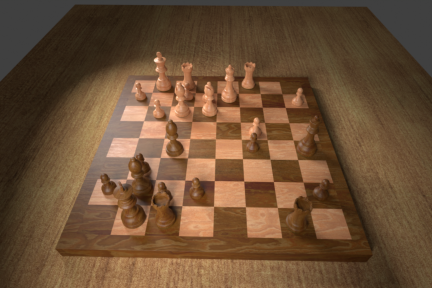
\includegraphics[width=\textwidth]{3828_corners_orig}
        \caption{original image}
    \end{subfigure}
    \hfill
    \begin{subfigure}[t]{0.47\textwidth}
        \centering
        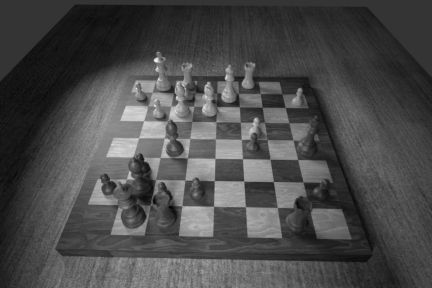
\includegraphics[width=\textwidth]{3828_corners_gray}
        \caption{grayscale image}
    \end{subfigure}
    
    \bigskip
    \begin{subfigure}[t]{0.47\textwidth}
        \centering
        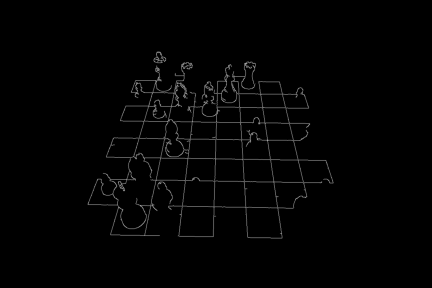
\includegraphics[width=\textwidth]{3828_corners_edges}
        \caption{detected edges}
        \label{fig:board_localisation_line_detection_edges}
    \end{subfigure}
    \hfill
    \begin{subfigure}[t]{0.47\textwidth}
        \centering
        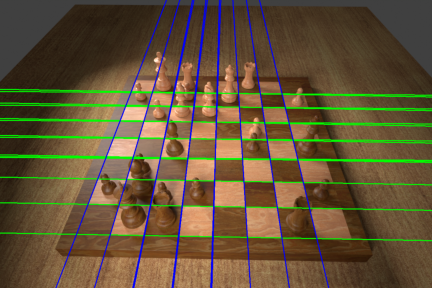
\includegraphics[width=\textwidth]{3828_corners_lines}
        \caption{detected lines, clustered into horizontal (green) and vertical (blue) lines}
        \label{fig:board_localisation_line_detection_horizontal_vertical}
    \end{subfigure}
    
    \bigskip
    \begin{subfigure}[t]{0.47\textwidth}
        \centering
        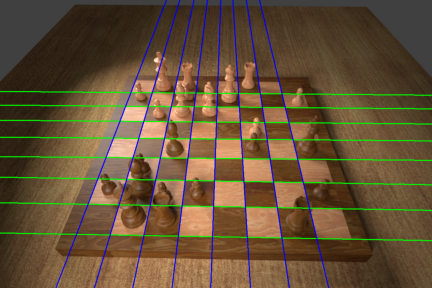
\includegraphics[width=\textwidth]{3828_corners_lines_clustered}
        \caption{elimination of similar lines}
        \label{fig:board_localisation_line_detection_elimination}
    \end{subfigure}
    \hfill
    \begin{subfigure}[t]{0.47\textwidth}
        \centering
        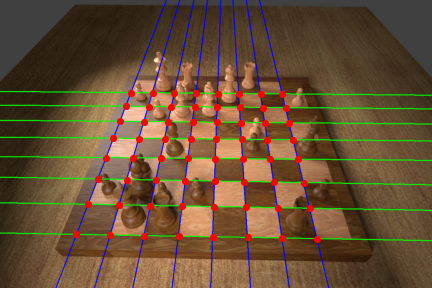
\includegraphics[width=\textwidth]{3828_corners_intersection_points}
        \caption{intersection points (red)}
        \label{fig:board_localisation_line_detection_intersections}
    \end{subfigure}
    \caption{The process of determining the intersection points on the chessboard.}
    \label{fig:board_localisation_line_detection}
\end{figure}
A chessboard consists of 64 squares that are arranged in an $8\times 8$ grid, thus there are nine horizontal and nine vertical lines.
In the first step of our algorithm, we would like to detect the majority of these lines and find their intersection points.

\paragraph{Edge detection}
To do so, we convert the \gls{rgb} image to grayscale and apply the Canny edge detector \cite{canny1986}, the result of which is shown in \cref{fig:board_localisation_line_detection_edges}.
Canny edge detection is a multi-stage algorithm that first reduces noise in the image by applying a Gaussian blur, then calculates pixel intensity gradients, performs non-maximum supression, and finally refines the results using hysteresis thresholding \cite{canny1986}, although the precise details of this algorithm go beyond the scope of this report.

\paragraph{Line detection}
\begin{figure}
    \centering
    \begin{tikzpicture}
        \begin{axis}[
            y dir = reverse,
            axis lines = center,
            xmin = 0, xmax = 4.5,
            ymin = 0, ymax = 2.5,
            xlabel = $x$,
            ylabel = $y$,
            xlabel style = {anchor=west},
            ylabel style = {anchor=north, at={(0,0)}},
            xtick = {0},
            ytick = {0},
            extra x ticks = 0,
            extra x tick style = {
                tick label style={
                    anchor=south east,
                    at={(-.1,-.1)}
            }},
            x=1cm,
            y=1cm,
            no markers
        ]
            \addplot {.5*-x + 2};
            \coordinate (O) at (0,0);
            \coordinate (A) at (.8,1.6);
            \coordinate (B) at (4,0);
            \draw[->] (O) -- (A) node[pos=.7,left] {$\rho$};
            \pic[draw, "$\theta$", <-, angle eccentricity=.6, angle radius=.7cm] {angle = A--O--B};
            \markRightAngle[size=8pt](B,A,O);
        \end{axis}
    \end{tikzpicture}
    \caption[A line in Hesse normal form.]{A line in Hesse normal form is parameterised by the angle $\theta$ to the $x$-axis and distance $\rho$ from the origin. The line is defined by the equation $\rho = x \cos \theta + y \sin \theta$. Equivalently, in slope-intercept form, we have $y = -x \cot \theta + \frac{\rho}{\sin \theta}$ provided that $\cos \theta \neq 0$, i.e. $\theta$ is not a multiple of $\pi$. Notice that the $y$-axis is pointing down because the origin of the coordinate system is the top left of the image.}
    \label{fig:hesse_normal_form}
\end{figure}
Next, we perform the so-called Hough transform \cite{hough1962,duda1972}, in order to detect lines that are formed by the edges.
To this end, we will represent lines in Hesse normal form, meaning that that they are parameterised by the angle $\theta$ that the normal vector makes to the $x$-axis, and the distance $\rho$ to the origin.
\Cref{fig:hesse_normal_form} explains this geometrically and gives rise to the equation of a line in Hesse normal form,
\begin{equation}
    \label{eq:hesse_normal_form}
    \rho = x \cos \theta + y \sin \theta.
\end{equation}
In fact, for a particular point $(x,y)$, \cref{eq:hesse_normal_form} represents the family of lines passing through it.
Here, each pair of $(\rho, \theta)$ values represents one particular line, and we only need to consider pairs where $\rho \geq 0$ and $0 \leq \theta < 2 \pi$ to parameterise all lines.

\begin{figure}
    \centering
    \begin{subfigure}[t]{0.4\textwidth}
        \begin{tikzpicture}
            \begin{axis}[
                y dir=reverse,
                xmin=0, 
                ymin=0, ymax=6,
                xlabel={$x$},
                ylabel={$y$},
                x=1cm,
                y=1cm
            ]
                \addplot+[mark=*] coordinates {(1,5)};
                \addplot+[mark=*] coordinates {(2,3)};
                \addplot+[mark=*] coordinates {(3,1)};
                \addplot[mark=none, dashed] {-2*x+7};
            \end{axis}
        \end{tikzpicture}
        \caption{three points in image space}
        \label{fig:hough_points_image_space}
    \end{subfigure}
    \hfill
    \begin{subfigure}[t]{0.56\textwidth}
        \begin{tikzpicture}
            \begin{axis}[
                no markers,
                xmin=0, xmax=6.28,
                ymin=0, ymax=6,
                samples=80,
                xlabel={$\theta$},
                ylabel={$\rho$},
                ylabel near ticks,
                yticklabel pos=right
            ]
                \addplot {1*cos(deg(x))+5*sin(deg(x))};
                \addplot {2*cos(deg(x))+3*sin(deg(x))};
                \addplot {3*cos(deg(x))+1*sin(deg(x))};
            \end{axis}
        \end{tikzpicture}
        \caption{lines passing through these three points in $(\rho,\theta)$ space}
        \label{fig:hough_points_parameter_space}
    \end{subfigure}
    \caption[An example of how lines in image space are represented in $(\rho,\theta)$ space.]{An example of how lines in image space are represented in $(\rho,\theta)$ space. The family of lines passing through a particular point in image space \subref{fig:hough_points_image_space} is represented by a sinusoid in $(\rho,\theta)$ space \subref{fig:hough_points_parameter_space}. The intersection point of the three curves represents the line passing through all three points.}
    \label{fig:hough_points}
\end{figure}
Plotting the pairs of $(\rho, \theta)$ values for a particular point in image space will give a sinusoidal curve that represents all lines passing through that point.
We can take multiple points in image space and plot their sinusoids. 
Then, each intersection in $(\rho, \theta)$ space will represent a line passing through the corresponding points, as illustrated in \cref{fig:hough_points}.

For a given threshold $t$, the Hough transform essentially plots the sinusoids for all edge points in the input image (which we obtained using the Canny edge detection algorithm) and outputs intersection points in $(\rho,\theta)$ space that are on at least $t$ different sinusoids.
Consequently, the lines identified by the Hough transform are corroborated by at least $t$ edge points in the image.

\paragraph{Clustering}
On the chessboard images, the Hough transform typically yields around 200 lines, most of which are very similar. 
We will first split them into horizontal and vertical lines and then eliminate similar lines.
Experiments showed that simply setting thresholds for the angle $\theta$ is insufficient for robustly classifying lines as horizontal or vertical.
This is because the camera is often tilted quite severely in the dataset (and might be the case in real chessboard photos taken by humans, too).
Instead, we employ agglomerative clustering which is a bottom-up hierarchical clustering algorithm.
In this algorithm, each line starts off in its own cluster, and as the algorithm progresses, pairs of clusters are merged in a manner that aims to minimise the variance within the clusters.
We cluster the lines based only on their direction, i.e. their angle $\theta$, and use the smallest angle between two given lines as the distance metric.
Finally, we use the mean angle of both top-level clusters to determine which cluster represents the vertical lines and which the horizontal lines.
The clustered lines are depicted in \cref{fig:board_localisation_line_detection_horizontal_vertical}.

Next, we must eliminate similar lines by finding clusters of similar lines.
To eliminate similar horizontal lines, we first find the mean vertical line by considering the $\rho$ and $\theta$ values associated to the lines in the vertical cluster.
Then, we find the intersection points of all the horizontal lines with the mean vertical line and perform a DBSCAN clustering \cite{ester1996} to group similar lines based on these intersection points.
We use the mean $\rho$ and $\theta$ values of the lines in each group to represent the final set of discovered horizontal lines. 
The same procedure is applied vice-versa for the vertical lines, the result of which is shown in \cref{fig:board_localisation_line_detection_elimination}.

\paragraph{Intersection points}
It remains to find the intersection points of the horizontal and vertical lines.
Given two lines parameterised by $(\rho_1,\theta_1)$ and $(\rho_2,\theta_2)$ respectively, we can find their point of intersection by observing that their equations in Hesse normal form (\cref{eq:hesse_normal_form}) forms a system of two linear equations that can be solved for $x$ and $y$. 
We have
\begin{align*}
    \rho_1 &= x \cos \theta_1 + y \sin \theta_1 \\
    \rho_2 &= x \cos \theta_2 + y \sin \theta_2.
\end{align*}
Rearranging for $x$ and $y$, we obtain after some algebraic manipulation
\begin{align}
    \label{eq:hesse_intersection_1}
    x &= \frac{\rho_2 \sin \theta_1 - \rho_1 \sin \theta_2}{\cos \theta_2 \sin \theta_1 - \cos \theta_1 \sin \theta_2}, \\
    \label{eq:hesse_intersection_2}
    y &= \frac{\rho_2 \cos \theta_1 - \rho_1 \cos \theta_2}{\sin \theta_2 \cos \theta_1 - \sin \theta_1 \cos \theta_2}.
\end{align}
Finally, using \cref{eq:hesse_intersection_1,eq:hesse_intersection_2} on each pair of horizontal and vertical lines, we can find the intersection points as depicted in \cref{fig:board_localisation_line_detection_intersections}.

\subsection{Finding the homography}
\subsection{Inferring missing lines}
\subsection{Determining optimal parameters}
The final stage of the edge detector (hysteresis) is parameterised by two threshold values 
Grid search

\section{Occupancy classification}
\label{sec:occupancy_classification}

Empirical experiments showed that performing piece classification directly after detecting the four corner points with no intermediate step yields a large number of false positives, i.e. empty squares being classified as containing a chess piece.
\begin{figure}
    \centering
    \begin{subfigure}[b]{0.65\textwidth}
        \centering
        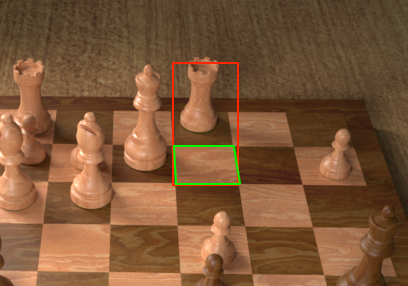
\includegraphics[width=\textwidth]{3828_annotated}
        \caption{region from the original image with marked square}
        \label{fig:occupancy_classification_fp_original}
    \end{subfigure}
    \hfill
    \begin{subfigure}[b]{0.3\textwidth}
        \centering
        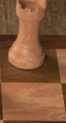
\includegraphics[width=.7\textwidth]{3828_cut}
        \caption{cropped sample}
        \label{fig:occupancy_classification_fp_cropped}
    \end{subfigure}
    \caption[An example illustraing why an immediate piece classification approach is inclined to reporting false positives.]{An example illustraing why an immediate piece classification approach is inclined to reporting false positives. Consider the square marked in green in the original image \subref{fig:occupancy_classification_fp_original}. The bounding box for piece classification (marked in red) must be quite tall because the square might contain a tall piece such as a queen or king (the box must be at least as tall as the the queen in the adjacent square on the left). The resulting sample, depicted in \subref{fig:occupancy_classification_fp_cropped}, contains almost the entire rook of the square behind. Thus, a piece classifier might classify this square as containing a rook instead of being empty.}
    \label{fig:occupancy_classification_fp}
\end{figure}
One common scenario where the trained classifier failed is illustrated in \cref{fig:occupancy_classification_fp}.
Notice that squares further away from the camera must be cropped with increasingly taller bounding boxes.
If a particular square is empty but its bounding box includes the piece from the adjacent square as in \cref{fig:occupancy_classification_fp_cropped}, the trained classifier was inclined to report a false positive.

To solve this problem, a binary classifier is trained on cropped squares to decide whether they are empty or not.
Before cutting out the squares from the original image, the input image is warped to a two-dimensional overhead view by means of a projective transformation.
This ensures that all squares are of equal size and that the corners form right angles (which is not the case in the original image due to perspective distortion).
To this end, we compute the \emph{homography matrix} $\mH \in \R^{3 \times 3}$ \cite{szeliski2011} mapping any point
$\vp$
from the original image to
the corresponding point
$\vp'$
in the warped image.
To simplify notation, we shall consider 2D homogenous coordinate vectors, i.e. three-component vectors with the last component being $1$, so the vector
$\begin{bmatrix}
    x & y & 1
\end{bmatrix}^\top$
would represent the point $(x,y)$ in the Cartesian coordinate system.
Using this notation, $\mH$ maps $\vp$ to $\vp'$ using the relation
\begin{equation}
    \label{eq:homography_matrix_relation}
    \mH
    \vp
    = s \vp'
\end{equation}
up to a scalar scale factor $s$.

Let the $4 \times 3$ matrix $\mP$ contain the pixel coordinates of the four chessboard corners starting in the top left in clockwise order and $\mP'$ be a matrix of the same size containing the corner coordinates of a square with side length $l$ pixels given by
\begin{equation*}
    \mP' = \begin{bmatrix}
        0 & l & l & 0 \\
        0 & 0 & l & l \\
        1 & 1 & 1 & 1
    \end{bmatrix}.
\end{equation*}
Notice that $\mP'$ describes a square whose top left corner is at the origin, and the coordinates are given in the same order as in $\mP$.
Since the homography matrix should map points from the original image to the output image, we obtain from \cref{eq:homography_matrix_relation} the relation 
\begin{equation}
    \label{eq:homography_matrix_relation_corners}
    \mH \mP = \mP' (\mI_4 \vs)
\end{equation}
where the vector $\vs \in \R^4$ represents the scale factor for each point.
\Cref{eq:homography_matrix_relation_corners} describes an overdetermined set of linear equations, so it is likely that there is no exact solution for $\mH$. 
However, we approximate $\mH$ by finding the solution with the least squared error.
Finally, we can use $\mH$ to apply the projective transformation to the original image such as depicted in \cref{fig:occupancy_classification_samples_original}, obtaining the warped image in \cref{fig:occupancy_classification_samples_warped}.
\begin{figure}
    \centering
    \begin{subfigure}[b]{0.47\textwidth}
        \centering
        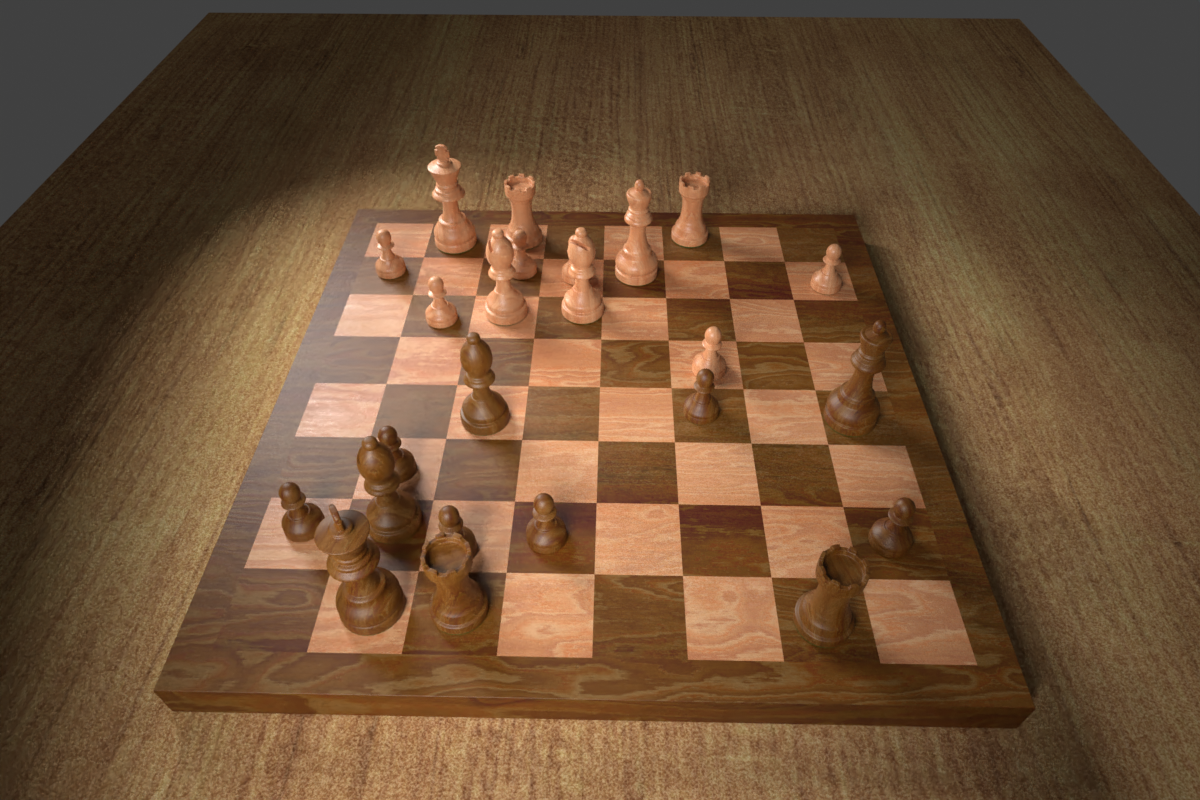
\includegraphics[width=\textwidth]{3828}
        \caption{original}
        \label{fig:occupancy_classification_samples_original}
    \end{subfigure}
    \hfill
    \begin{subfigure}[b]{0.47\textwidth}
        \centering
        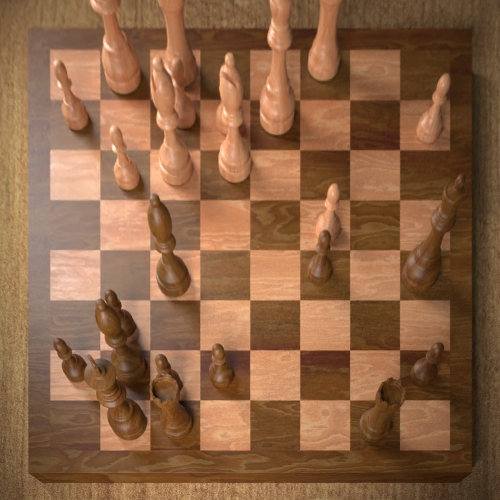
\includegraphics[width=\textwidth]{3828_unwarped}
        \caption{warped}
        \label{fig:occupancy_classification_samples_warped}
    \end{subfigure}
    
    \bigskip
    \begin{subfigure}[b]{0.47\textwidth}
        \centering
        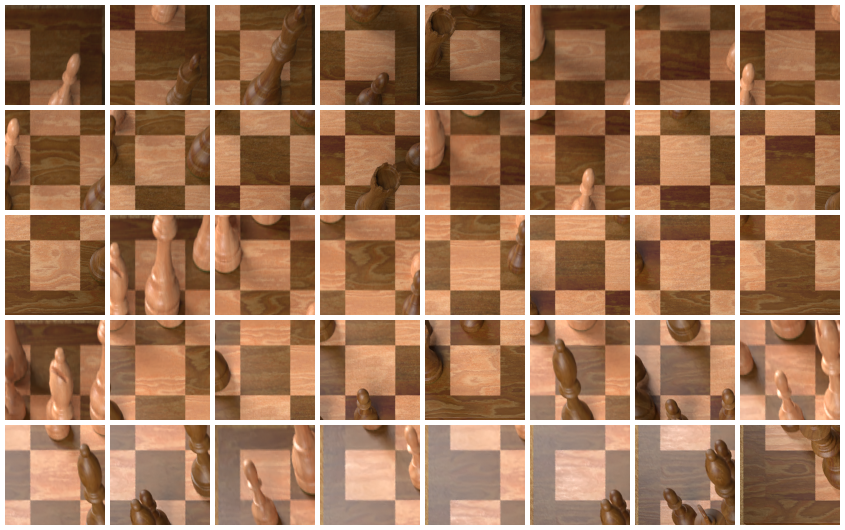
\includegraphics[width=\textwidth]{3828_empty}
        \caption{all 32 empty samples}
        \label{fig:occupancy_classification_samples_empty}
    \end{subfigure}
    \hfill
    \begin{subfigure}[b]{0.47\textwidth}
        \centering
        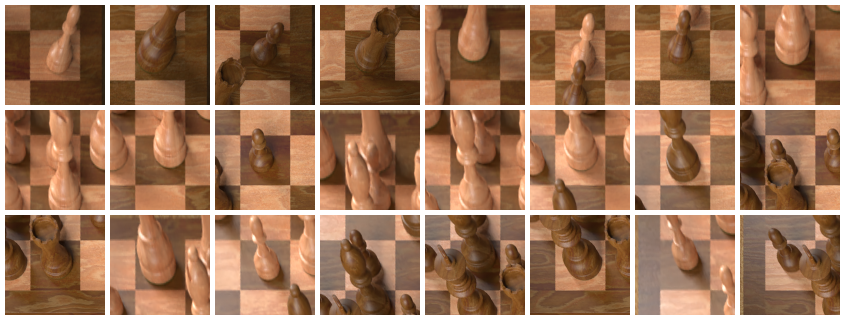
\includegraphics[width=\textwidth]{3828_occupied}
        \caption{all 24 occupied samples}
        \label{fig:occupancy_classification_samples_occupied}
    \end{subfigure}
    \caption[The process of obtaining samples for occupancy classification from a chessboard image.]{The process of obtaining samples for occupancy classification from a chessboard image. First, the original image \subref{fig:occupancy_classification_samples_original} is warped to a two-dimensional overhead view, \subref{fig:occupancy_classification_samples_warped}. Then, all squares are cropped (with a 50\% increase in width and height to include contextual information). Finally, the cropped squares are annoted using the \gls{fen} groundtruth as either empty \subref{fig:occupancy_classification_samples_empty} or occupied \subref{fig:occupancy_classification_samples_occupied}.}
    \label{fig:occupancy_classification_samples}
\end{figure}

Cropping the squares from the warped image is trivial because the squares are of equal size.
In training the occupancy classifiers, it is conjectured that it would be useful to include contextual information with each square; therefore, the squares are not cropped tightly around their boundaries but instead with a 50\% increase in length on all four sides, as shown in \cref{fig:occupancy_classification_samples_empty,fig:occupancy_classification_samples_occupied}.
This might aid the classifier's decision in difficult situations where a chess piece from another square reaches into the cropped one due to the camera perspective.

\subsection{Training \glspl{cnn}}
Six \gls{cnn} architectures are devised for the occupancy classification task, of which two accept $100\times 100$ pixel input images and the remaining four require the images to be of size $50\times 50$ pixels.
They differ in the number of convolution layers, pooling layers, and fully connected layers.
When referring to these models, we shall use a 4-tuple consisting of the input side length and the three aforementioned criteria.
\Cref{fig:occupancy_convnet} depicts the architecture of the \gls{cnn} $(100, 3, 3, 3)$ model which achieves the greatest validation accuracy of these six models.
\begin{figure}
    \centering
    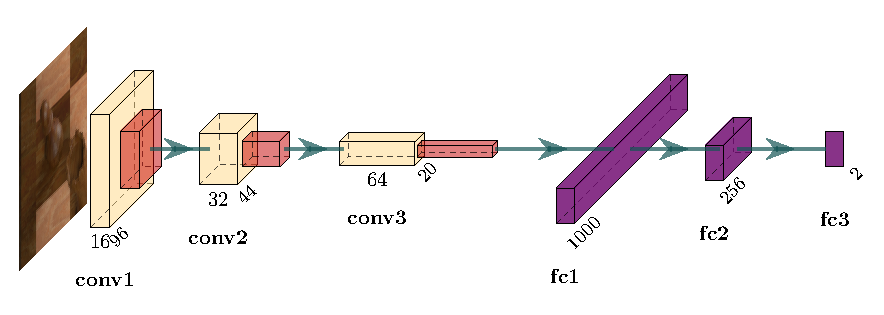
\includegraphics[width=\textwidth]{occupancy_convnet}
    \caption[Architecture of the CNN $(100,3,3,3)$ network for occupancy classification.]{
        Architecture of the \gls{cnn} $(100,3,3,3)$ network for occupancy classification.
        The input is a three-channel \gls{rgb} image with $100\times 100$ pixels.
        There are two convolutional layers (yellow) with a kernal size of $5 \times 5$ and stride $1$, meaning that each convolutional layer reduces the width and height by $4$.
        The final convolutional layer has a kernel size of $3 \times 3$, thus only reducing the input size by two.
        Starting with 16 filters in the first convolutional layer, the number of channels is doubled in each subsequent layer, as is common practice in \glspl{cnn} \cite{simonyan2015}.
        Each convolutional layer uses the \gls{relu} activation function and is followed by a max pooling layer with a $2\times 2$ kernel that is moved with a stride of $2$ such that the width and height are halved.
        Finally, the output of the last pooling layer is reshaped to a 640,000-dimensional vector that passes through two fully connected \gls{relu}-activated layers before reaching the final fully connected layer with softmax activation.
    }
    \label{fig:occupancy_convnet}
\end{figure}
The final fully connected layer in each model contains two output units that represent the two classes (occupied and empty).
The models are trained using the cross-entropy loss function on the outputs.
Training proceeds using the popular \emph{Adam} optimizer \cite{kingma2017} with a learning rate of $0.001$ for three whole passes over the training set using a batch size of 128.
After every 100 steps, the model's loss and accuracy is computed over the entire validation set, the results of which are reported in \cref{fig:occupancy_cnn_loss_accuracy}.
\begin{figure}
    \makebox[\textwidth][c]{
        \begin{subfigure}{.45\textwidth}
            \begin{tikzpicture}
                \begin{axis}[
                    no markers,
                    xlabel={step},
                    ylabel={cross-entropy loss},
                    title={Loss},
                    scale only axis,
                    width=.9\textwidth,
                    legend style={at={(0.98,0.98)},anchor=north east}
                ]
                    \addplot table [x=Step, y=Value, col sep=comma] {data/run-occupancy_classifier_CNN100_3Conv_3Pool_3FC_train-tag-Loss.csv};
                    \addplot table [x=Step, y=Value, col sep=comma] {data/run-occupancy_classifier_CNN100_3Conv_3Pool_3FC_val-tag-Loss.csv};
                    \legend{training,validation}
                \end{axis}
            \end{tikzpicture}
        \end{subfigure}
        \hfill
        \begin{subfigure}{.45\textwidth}
            \begin{tikzpicture}
                \begin{axis}[
                    no markers,
                    xlabel={step},
                    ylabel={accuracy},
                    title={Accuracy},
                    scale only axis,
                    width=.9\textwidth,
                    ylabel near ticks,
                    yticklabel pos=right,
                    legend style={at={(0.98,0.02)},anchor=south east}
                ]
                    \addplot table [x=Step, y=Value, col sep=comma] {data/run-occupancy_classifier_CNN100_3Conv_3Pool_3FC_train-tag-Accuracy.csv};
                    \addplot table [x=Step, y=Value, col sep=comma] {data/run-occupancy_classifier_CNN100_3Conv_3Pool_3FC_val-tag-Accuracy.csv};
                    \legend{training,validation}
                \end{axis}
            \end{tikzpicture}
        \end{subfigure}
    }
    \caption[Loss and accuracy during training on both the training and validation sets for the CNN $(100,3,3,3)$ model.]{Loss and accuracy during training on both the training and validation sets for the \gls{cnn} $(100,3,3,3)$ model. The best validation accuracy is 99.71\%.}
    \label{fig:occupancy_cnn_loss_accuracy}
\end{figure}
The model converges smoothly to a very low loss value, achieving a training accuracy of 99.70\% and validation accuracy of 99.71\%.
Due to the fact that the difference between training and validation accuracy is very small (in fact, the validation accuracy even happens to be slightly above the training accuracy), we conclude that the model does not overfit the training set.

\subsection{Transfer learning on deeper models}
VGG \cite{simonyan2015}
ResNet \cite{he2016}
AlexNet \cite{krizhevsky2017}
ImageNet \cite{deng2009}


\todo{todo: explain how this was done and explain tradeoff (significantly more parameters in model)}

\subsection{Analysis}
Each model is trained separately on the dataset of squares that are cropped to include contextual information (by increasing the bounding box by 50\% in each direction), and the same samples except that the squares are cropped tightly.
In each case, the model trained on the samples that contained contexual information outperfomed its counterpart trained on tightly cropped samples, confirming the hypothesis that the information around the square itself is useful.


\begin{table}
    \centering
    \makebox[\textwidth][c]{
        \pgfplotstabletypeset[
            col sep=tab,
            columns={context,model,parameters,val_accuracy,val_precision/occupied,val_recall/occupied,val_misclassified,train_accuracy},
            every head row/.style={%
                before row=\toprule,
                after row=\midrule%
            },
            every last row/.style={
                after row=\bottomrule
            },
            columns/model/.style={
                string type
            },
            columns/context/.style={
                string type,
                column name={}
            },
            columns/val_accuracy/.style={
                dec sep align,
                postproc cell content/.append code={
                    \ifnum1=\pgfplotstablepartno
                        \pgfkeysalso{@cell content/.add={}{\%}}%
                    \fi
                },
                fixed,
                fixed zerofill,
                column name={accuracy}
            },
            columns/train_accuracy/.style={
                dec sep align,
                postproc cell content/.append code={
                    \ifnum1=\pgfplotstablepartno
                        \pgfkeysalso{@cell content/.add={}{\%}}%
                    \fi
                },
                fixed,
                fixed zerofill,
                column name={\makecell{training \\ accuracy}}
            },
            columns/val_precision/occupied/.style={
                dec sep align,
                precision=3,
                fixed,
                fixed zerofill,
                column name={precision}
            },
            columns/val_recall/occupied/.style={
                dec sep align,
                precision=3,
                fixed,
                fixed zerofill,
                column name={recall}
            },
            columns/val_misclassified/.style={
                column name={\makecell{errors}}
            },
        ]{data/occupancy_classifier.dat}
    }
    \caption[Performance of all occupancy classification models on the validation set.]{
        Performance of all occupancy classification models on the validation set.
        For the \gls{cnn} models, the 4-tuple denotes the length of the square input size in pixels, the number of convolution layers, the number of pooling layers, and the number of fully connected layers.
        The check mark in the left column indicates whether the input samples contained contextual information (cropped to include part of the adjacent squares).
        In the penultimate column, the total number of misclassifications in the validation set are reported (the validation set consists of 9,346 samples).
        The training accuracy is given in the rightmost column for comparison.
        Notice that there is no significant difference between the validation and training accuracies, indicating that none of the models suffer from overfitting.
    }
\end{table}

\begin{figure}
    \makebox[\textwidth][c]{
        \begin{subfigure}{.45\textwidth}
            \begin{tikzpicture}
                \begin{axis}[
                    no markers,
                    xlabel={step},
                    ylabel={cross-entropy loss},
                    title={Loss},
                    scale only axis,
                    width=.9\textwidth,
                    legend style={at={(0.98,0.98)},anchor=north east}
                ]
                    \addplot table [x=Step, y=Value, col sep=comma] {data/run-occupancy_classifier_ResNet_train-tag-Loss.csv};
                    \addplot table [x=Step, y=Value, col sep=comma] {data/run-occupancy_classifier_ResNet_val-tag-Loss.csv};
                    \legend{training,validation}
                \end{axis}
            \end{tikzpicture}
        \end{subfigure}
        \hfill
        \begin{subfigure}{.45\textwidth}
            \begin{tikzpicture}
                \begin{axis}[
                    no markers,
                    xlabel={step},
                    ylabel={accuracy},
                    title={Accuracy},
                    scale only axis,
                    width=.9\textwidth,
                    ylabel near ticks,
                    yticklabel pos=right,
                    legend style={at={(0.98,0.02)},anchor=south east}
                ]
                    \addplot table [x=Step, y=Value, col sep=comma] {data/run-occupancy_classifier_ResNet_train-tag-Accuracy.csv};
                    \addplot table [x=Step, y=Value, col sep=comma] {data/run-occupancy_classifier_ResNet_val-tag-Accuracy.csv};
                    \legend{training,validation}
                \end{axis}
            \end{tikzpicture}
        \end{subfigure}
    }
    \caption[Loss and accuracy during training on both the training and validation sets for the ResNet model.]{Loss and accuracy during training on both the training and validation sets for the ResNet model. The best validation accuracy is 99.96\%.}
    \label{fig:occupancy_resnet_loss_accuracy}
\end{figure}

\begin{figure}
    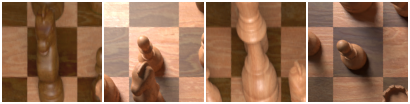
\includegraphics[width=\textwidth]{ResNet_val_mistakes.png}
    \caption[The four samples that the ResNet model misclassified in the validation set.]{The four samples that the ResNet model misclassified in the validation set. The left sample depicts an empty square, and the remaining three are of occupied squares.}
    \label{fig:occupancy_resnet_mistakes}
\end{figure}

\section{Piece classification}
\label{sec:piece_classification}
Now that the occupancy of each square on the chessboard can be detected to a high degree of accuracy, the next step is to classify the piece in each of the occupied squares.
We require a 12-way classifier that takes as input a cropped image of an occupied square and will output the chess piece on that square. 
There are six types of chess pieces (pawn, knight, bishop, rook, queen, and king), and each piece can either be white or black in colour, thus there are 12 classes of pieces.

We must pay some special attention to how the pieces are cropped. 
Simply following the approach described in \cref{sec:occupancy_classification} for cropping squares does not give enough information to classify pieces.
Especially tall pieces at the back of the board would be cropped in a manner such that only the bottom part of the piece remains in the \gls{roi}. 
Consider for example the white king in \cref{fig:occupancy_classification_samples}.
Cropping only the square it is located in would not include its crown which is an important feature needed to distinguish between kings and queens.
Instead, we must choose a rectangular bounding box that is tall enough to account for the perspective distortion.

The camera perspective causes another phenomenon that we must account for: pieces on the left of the board tend to `slant' to the left, and vice-versa on the right.
This is due to the vanishing point of the normal vectors on the chessboard surface being roughly centred horizontally with regards to the location of the chessboard itself%
\footnote{%
    Unfortunately, it is not possible to compute the vanishing point of the normals based solely on the information available in the input images as this would require knowledge of the intrinsic and extrinsic camera parameters \cite{hartley2004}.
    The aim of this work is to recognise chess positions from just the input image without any further information; therefore, we devise a heuristic based on the observation that the vanishing point tends to be vertically below the chessboard and roughly horizontally centred.
}, as illustrated in \cref{fig:occupancy_classification_normals}.
\begin{figure}
    \centering
    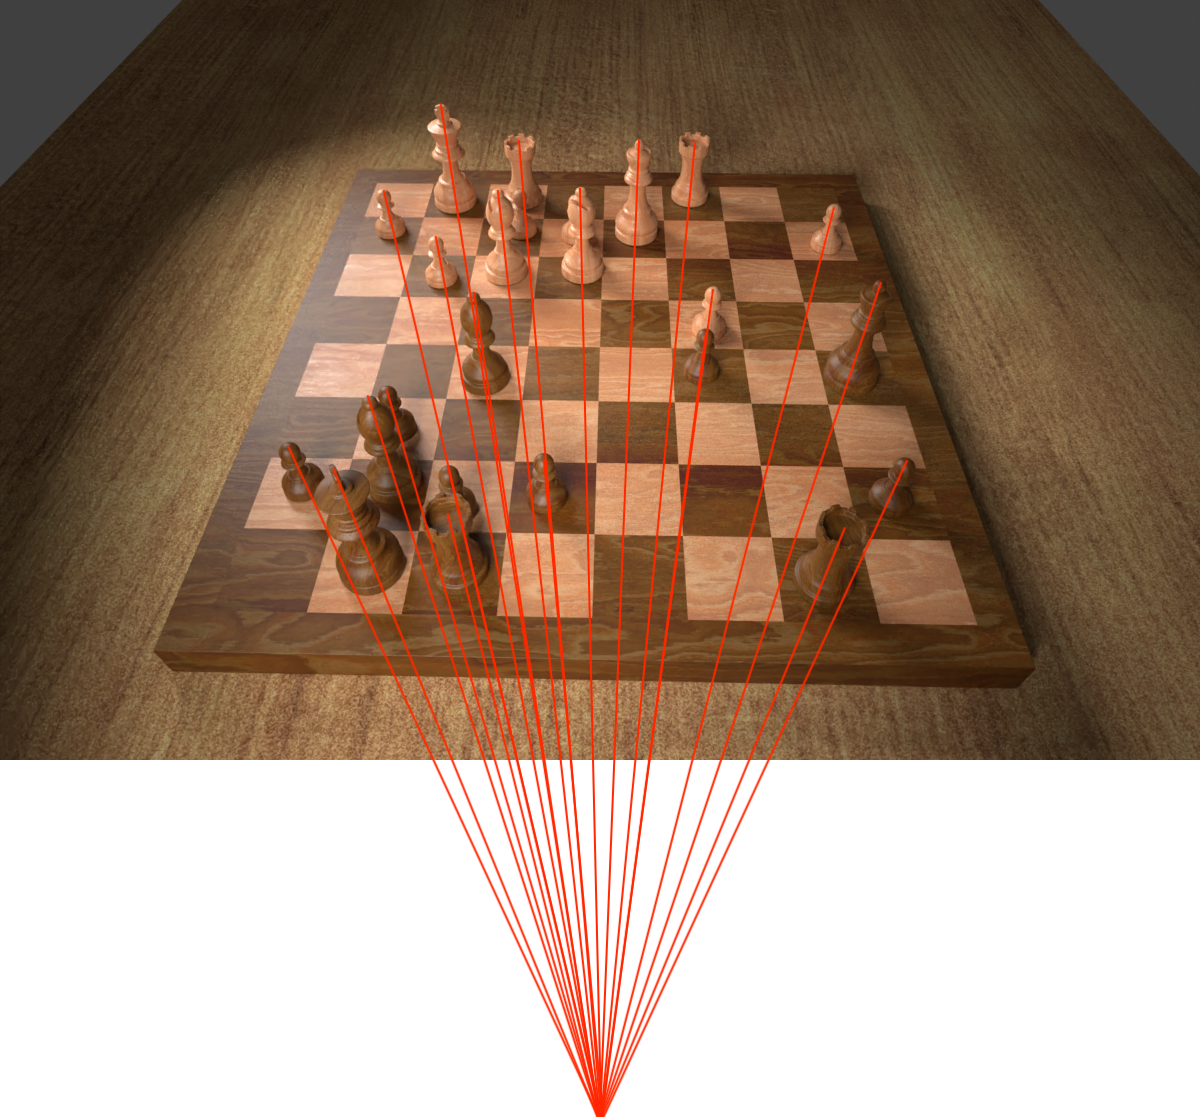
\includegraphics[width=.7\textwidth]{3828_normals.png}
    \caption[The normals of the chessboard surface converge to a single vanishing point which is below the image.]{The normals of the chessboard surface (corresponding to the direction the pieces are pointing, marked in red) converge to a single vanishing point which is below the image. We will assume that the vanishing point is roughly horizontally centred with the chessboard, as this corresponds to how chessboards are usually photographed. As a result, pieces on left `lean' left, and vice-versa on the right.}
    \label{fig:occupancy_classification_normals}
\end{figure}
Hence, we must extend the \gls{roi} vertically in the appropriate direction.

To obtain the \glspl{roi}, we first warp the input image of the chessboard as described in \cref{sec:occupancy_classification} and exemplified in \cref{fig:occupancy_classification_samples_warped}.
At first, each pieces bounding box will correspond to the square it is located on, i.e. its width and height will be that of the square\footnote{Note that due to the warped perspective, all squares have equal width and height.}.
Depending on the rank $r$, the height is increased by
\begin{equation*}
    h_\text{inc}(r) = \frac{2r + 5}{7}
\end{equation*}
where the unit of measurement is the height of the chessboard squares.
This represents an arithmetic progression such that the bounding box for pieces in the first rank (bottom row of the chessboard, i.e. $r=1$) will be increased by one square, and pieces in the top row ($r=8$) will have their height increased by three units.

The increase in width is dependent on the file $f$ and given by the piecewise-defined arithmetic progression
\begin{equation*}
    w_\text{inc}(f) = \begin{cases}
        -\frac{f}{4} & f \leq 4 \\
        \frac{f-4}{4} & f > 4.
    \end{cases}
\end{equation*}
A negative increase in width means that the bounding box is extended to the left, whereas a positive increase means it is widened to the right.
Thus, pieces on the left half of the board ($1 \leq f \leq 4$) will have their bounding boxes extended to the left, and vice-versa on the right (for $4 < f \leq 8$).

Experiments demonstrate that this heuristic generates bounding boxes that are large enough to contain even the tallest pieces in most cases, whilst not being needlessly large.
As a further preprocessing step, the cropped \glspl{roi} for all pieces on the left side of the board ($1 \leq f \leq 4$) are flipped vertically, such that the square that the piece stands on will always be in the bottom left of the image.
This may help the classifier understand what piece is being referred to in samples where the larger bounding box includes adjacent pieces in the image.
\Cref{fig:white_queens} shows a random selection of the \glspl{roi} corresponding to white queens in order to demonstrate that the bounding boxes are large enough to contain even tall pieces.
\begin{figure}
    \centering
    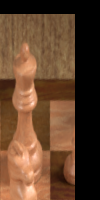
\includegraphics[width=.15\textwidth]{white_queen_1.png}
    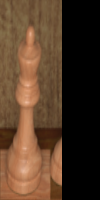
\includegraphics[width=.15\textwidth]{white_queen_2.png}
    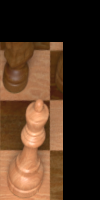
\includegraphics[width=.15\textwidth]{white_queen_3.png}
    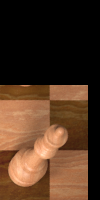
\includegraphics[width=.15\textwidth]{white_queen_4.png}
    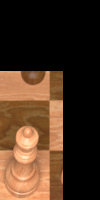
\includegraphics[width=.15\textwidth]{white_queen_5.png}
    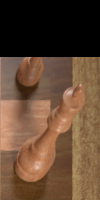
\includegraphics[width=.15\textwidth]{white_queen_6.png}
    \caption[A random selection of six samples of white queens in the training set.]{A random selection of six samples of white queens in the training set. Notice that the square each queen is located on is always in the bottom left of the image and of uniform dimensions across all samples.}
    \label{fig:white_queens}
\end{figure}

\subsection{Training \glspl{cnn}}
Similar to \cref{sec:occupancy_classification}, we train several models on 
\todo{talk about change in number of epochs etc}

\begin{figure}
    \makebox[\textwidth][c]{
        \begin{subfigure}{.45\textwidth}
            \begin{tikzpicture}
                \begin{axis}[
                    no markers,
                    xlabel={step},
                    ylabel={cross-entropy loss},
                    title={Loss},
                    scale only axis,
                    width=.9\textwidth,
                    legend style={at={(0.98,0.98)},anchor=north east}
                ]
                    \addplot table [x=Step, y=Value, col sep=comma] {data/run-piece_classifier_InceptionV3_train-tag-Loss.csv};
                    \addplot table [x=Step, y=Value, col sep=comma] {data/run-piece_classifier_InceptionV3_val-tag-Loss.csv};
                    \legend{training,validation}
                \end{axis}
            \end{tikzpicture}
        \end{subfigure}
        \hfill
        \begin{subfigure}{.45\textwidth}
            \begin{tikzpicture}
                \begin{axis}[
                    no markers,
                    xlabel={step},
                    ylabel={accuracy},
                    title={Accuracy},
                    scale only axis,
                    width=.9\textwidth,
                    ylabel near ticks,
                    yticklabel pos=right,
                    legend style={at={(0.98,0.02)},anchor=south east}
                ]
                    \addplot table [x=Step, y=Value, col sep=comma] {data/run-piece_classifier_InceptionV3_train-tag-Accuracy.csv};
                    \addplot table [x=Step, y=Value, col sep=comma] {data/run-piece_classifier_InceptionV3_val-tag-Accuracy.csv};
                    \legend{training,validation}
                \end{axis}
            \end{tikzpicture}
        \end{subfigure}
    }
    \caption[Loss and accuracy during training on both the training and validation sets for the InceptionV3 model.]{Loss and accuracy during training on both the training and validation sets for the InceptionV3 model. The best validation accuracy is 100.00\%.}
    \label{fig:pieces_inception_loss_accuracy}
\end{figure}

\begin{table}
    \centering
    \makebox[\textwidth][c]{
        \pgfplotstabletypeset[
            col sep=tab,
            columns={model,parameters,val_accuracy,val_misclassified,train_accuracy},
            every head row/.style={%
                before row=\toprule,
                after row=\midrule%
            },
            every last row/.style={
                after row=\bottomrule
            },
            columns/model/.style={
                string type
            },
            columns/val_accuracy/.style={
                dec sep align,
                postproc cell content/.append code={
                    \ifnum1=\pgfplotstablepartno
                        \pgfkeysalso{@cell content/.add={}{\%}}%
                    \fi
                },
                fixed,
                fixed zerofill,
                column name={accuracy}
            },
            columns/train_accuracy/.style={
                dec sep align,
                postproc cell content/.append code={
                    \ifnum1=\pgfplotstablepartno
                        \pgfkeysalso{@cell content/.add={}{\%}}%
                    \fi
                },
                fixed,
                fixed zerofill,
                column name={\makecell{training \\ accuracy}}
            },
            columns/val_misclassified/.style={
                column name={\makecell{errors}}
            },
        ]{data/piece_classifier.dat}
    }
    \caption[Performance of all piece classifiers on the validation set.]{
        Performance of all piece classifiers on the validation set.
    }
\end{table}

\section{Preparing the results}
\label{sec:preparing_results}

\end{document}